\documentclass[12pt]{beamer}
\usetheme{Warsaw}
\usepackage[utf8]{inputenc}
\usepackage[spanish]{babel}
\usepackage{amsmath}
\usepackage{amsfonts}
\usepackage{amssymb}
\usepackage{graphicx}
\usepackage{color}
\definecolor{softgray}{rgb}{0.8,0.8,0.8}
\usepackage{listings} %Para codigo
\author{Daniel Bolaños Martínez, José María Borrás Serrano, Santiago De Diego De Diego, Fernando De la Hoz Moreno}
\title{Práctica 2: Algoritmos Divide y Vencerás}
\setbeamercovered{transparent} 
\setbeamertemplate{navigation symbols}{} 
%\logo{} 
\institute{ETSIIT} 
\date{} 

%\subject{} 
\begin{document}

\begin{frame}
\titlepage
\end{frame}

\begin{frame}{Introducción}
Nos ha tocado resolver el ejercicio serie unimodal de números.

\vspace{5mm} %5mm vertical space

Para ello, hemos diseñado un algoritmo basado en “divide y vencerás” el cual tiene como objetivo encontrar el valor máximo de una serie unimodal. El orden de eficiencia de este algoritmo es $O(log(n))$ y lo hemos comparado con el algoritmo trivial para este problema que es de orden $O(n)$.
\end{frame}
\begin{frame}{Desarrollo de la Práctica}
Para la comparación hemos obtenido unas tablas en las que se muestran el tiempo de ejecución según distintos número de elementos en los vectores, hemos representado los datos en una gráfica y hemos ajustado estos datos a la función obtenida por la eficiencia teórica por el ajuste de mínimos cuadrados.
\end{frame}

\begin{frame}[fragile]{Código Divide y Vencerás}
	\lstset{language=C++, breaklines=true, extendedchars=true,backgroundcolor=\color{softgray}, keywordstyle=\color{blue},stringstyle=\color{orange},caption={Función unimodal DyV}, basicstyle=\tiny}
	\begin{lstlisting}
int unimodal(vector<int> v)
{
	bool fin=false;
	int maximo=v.size()-1;
	int indice=maximo/2;
	int minimo;
 
	while(!fin)
	{
        if(v.at(indice-1)<v.at(indice))
           if(v.at(indice+1)<v.at(indice))
			    fin=true;
		   else
		   {
				minimo=indice;
				indice=indice+((maximo-indice)/2);
			}
		else
		{
			maximo=indice;
			indice=minimo+((indice-minimo)/2);
		}
	}
	return indice;
}
	\end{lstlisting}
\end{frame}
\begin{frame}[fragile]
	\lstset{language=C++, breaklines=true, extendedchars=true, caption={Función main DyV},backgroundcolor=\color{softgray},keywordstyle=\color{blue},stringstyle=\color{orange},basicstyle=\tiny}
	\begin{lstlisting}
int main(int argc, char* argv[])
{
	vector<int> array;
  	int valor = -1;
	double suma=0;

	int v_size = atoi(argv[1]);
	array.resize(v_size);

	for(int i=0; i<100; ++i)
	{
		int p = 1 + rand() % (v_size-2);
  		array.at(p) = v_size-1;
  		for (int i=0; i<p; i++)
  			array.at(i)=i;
  		for (int i=p+1; i<v_size; i++)
  			array.at(i)=v_size-1-i+p;

		clock_t tantes;
		clock_t tdespues;
		tantes=clock();
		valor = unimodal(array);
		tdespues=clock();
		suma += (double)(tdespues - tantes) / CLOCKS_PER_SEC;
	}
  	cout << v_size <<" "<< suma/100 << endl;
}
	\end{lstlisting}

\end{frame}

\begin{frame}[fragile]{Código secuencial}
	\lstset{language=C++, breaklines=true, extendedchars=true,backgroundcolor=\color{softgray}, keywordstyle=\color{blue},stringstyle=\color{orange},caption={Función unimodal Secuencial}, basicstyle=\footnotesize}
	\begin{lstlisting}
int unimodal_secuencial(vector<int> v)
{
	bool fin=false;
  	int indice=1;

  	while(!fin)
  	{
     	if(v.at(indice+1)<v.at(indice))
      		fin=true;
     	else
      		indice++;
  	}

  	return indice;
}
	\end{lstlisting}
\end{frame}

\begin{frame}[fragile]
	\lstset{language=C++, breaklines=true, extendedchars=true, caption={Función main Secuencial},backgroundcolor=\color{softgray},keywordstyle=\color{blue},stringstyle=\color{orange},basicstyle=\tiny}
	\begin{lstlisting}
int main(int argc, char* argv[])
{
	vector<int> array;
  	int valor = -1;
	double suma=0;

  	int v_size = atoi(argv[1]);
  	array.resize(v_size);

	for(int i=0; i<100; ++i)
	{
		int p = 1 + rand() % (v_size-2);
  		array.at(p) = v_size-1;
  		for (int i=0; i<p; i++)
  			array.at(i)=i;
  		for (int i=p+1; i<v_size; i++)
  			array.at(i)=v_size-1-i+p;

  		clock_t tantes;
  		clock_t tdespues;
  		tantes=clock();
  		valor = unimodal_secuencial(array);
  		tdespues=clock();
		suma += (double)(tdespues - tantes) / CLOCKS_PER_SEC;
	}
  	cout << v_size <<" "<< suma/100 << endl;
}
	\end{lstlisting}

\end{frame}

\begin{frame}{Tabla Datos DyV}
\begin{tabular}{|c|c|c|}
\hline 
Tamaño Vectores & Tiempo Divide y Vencerás \\ 
\hline 
1048576 & 7.796e-05 \\ 
\hline 
2097152 & 0.00016308  \\ 
\hline 
4194304 & 0.00038871  \\ 
\hline 
8388608 & 0.00117717  \\ 
\hline 
16777216 & 0.00227126  \\ 
\hline 
33554432 & 0.00456919  \\ 
\hline 
67108864 & 0.00894183  \\ 
\hline 
134217728 & 0.0170173  \\ 
\hline 
268435456 & 0.0335588 \\ 
\hline 
536870912 & 0.0668834 \\ 
\hline 
\end{tabular} 

\end{frame}

\begin{frame}{Tabla Datos Secuencial}
\begin{tabular}{|c|c|}
\hline 
Tamaño Vectores & Tiempo Secuencial \\ 
\hline 
1000000 & 0.00169148 \\ 
\hline 
2000000 & 0.00341387 \\ 
\hline 
3000000 & 0.00515229 \\ 
\hline 
4000000 & 0.00688878 \\ 
\hline 
5000000 & 0.00583811 \\ 
\hline 
6000000 & 0.0102687 \\ 
\hline 
7000000 & 0.0119547 \\ 
\hline 
8000000 & 0.013579 \\ 
\hline 
9000000 & 0.0157071 \\ 
\hline 
10000000 & 0.017487 \\ 
\hline 
11000000 & 0.0192033 \\ 
\hline 
12000000 & 0.0209426 \\ 
\hline
\end{tabular}
\end{frame}

\begin{frame}
\begin{tabular}{|c|c|}
\hline 
Tamaño Vectores & Tiempo Secuencial \\
\hline
13000000 & 0.022794 \\ 
\hline 
14000000 & 0.0245116 \\ 
\hline 
15000000 & 0.0260875 \\ 
\hline 
16000000 & 0.0278383 \\ 
\hline 
17000000 & 0.0296462 \\ 
\hline 
18000000 & 0.0314487 \\ 
\hline 
19000000 & 0.033057 \\ 
\hline 
20000000 & 0.0348266 \\ 
\hline 
21000000 & 0.0367226 \\ 
\hline 
22000000 & 0.0383142 \\ 
\hline 
23000000 & 0.0401301 \\ 
\hline 
24000000 & 0.0418608 \\ 
\hline 
25000000 & 0.0434716 \\ 
\hline 
26000000 & 0.0455227 \\ 
\hline 
\end{tabular} 
\end{frame}

\begin{frame}{Eficiencia en el caso secuencial}

\begin{figure}[H] 
\centering
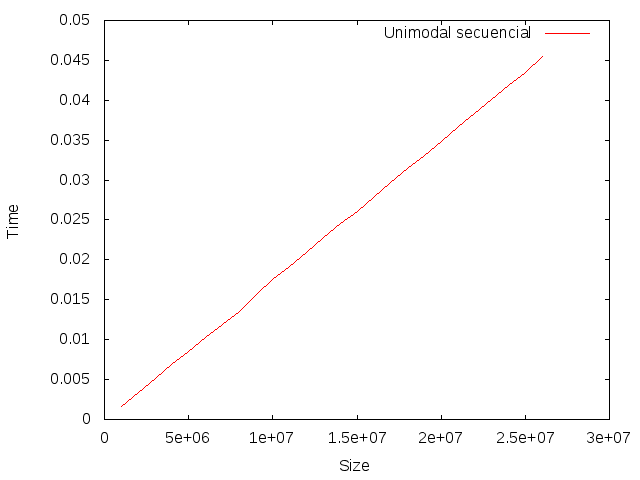
\includegraphics[angle=0,scale=0.5]{img/Eficiencia_sec.png} 
\end{figure}

\end{frame}

\begin{frame}{Eficiencia en el caso Divide y Vencerás}

\begin{figure}[H] 
\centering
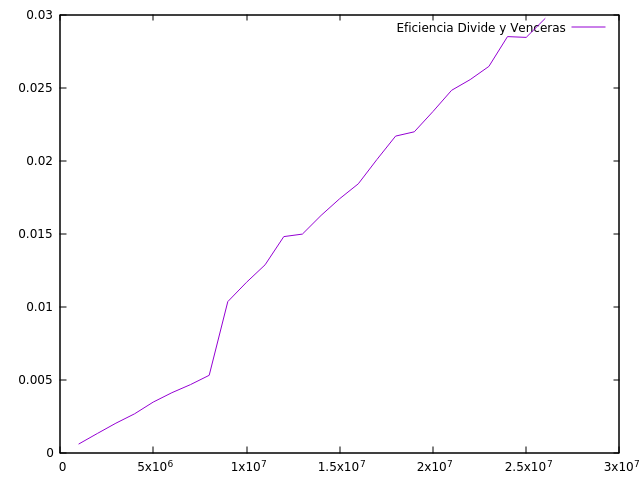
\includegraphics[angle=0,scale=0.5]{img/Eficiencia_dyv.png} 
\end{figure}

\end{frame}

\begin{frame}{Ajuste híbrido en el caso secuencial}

\begin{figure}[H] 
\centering
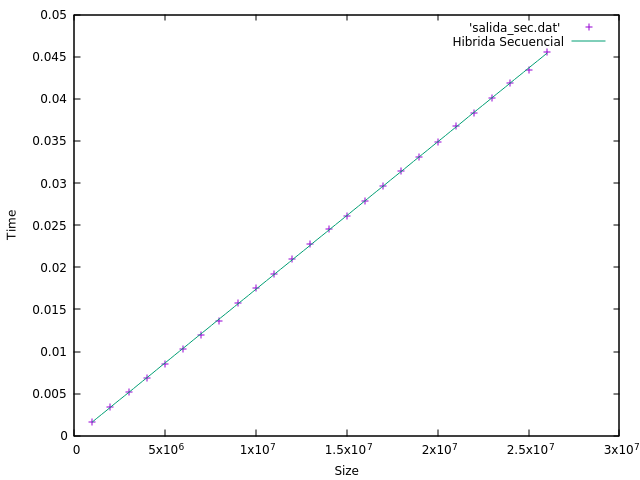
\includegraphics[angle=0,scale=0.5]{img/AjusteHibridoSec.png} 
\caption{Ajustada a la función $f(x)=a_0*x+a_1$} 
\end{figure}

\end{frame}

\begin{frame}
\[
f(x)=a_0*x+a_1 
\]
\[
a_0=1.75072e-09
\]
\[
a_1=-0.000131396
\]
\end{frame}

\begin{frame}{Ajuste híbrido en el caso Divide y Vencerás}

\begin{figure}[H] 
\centering
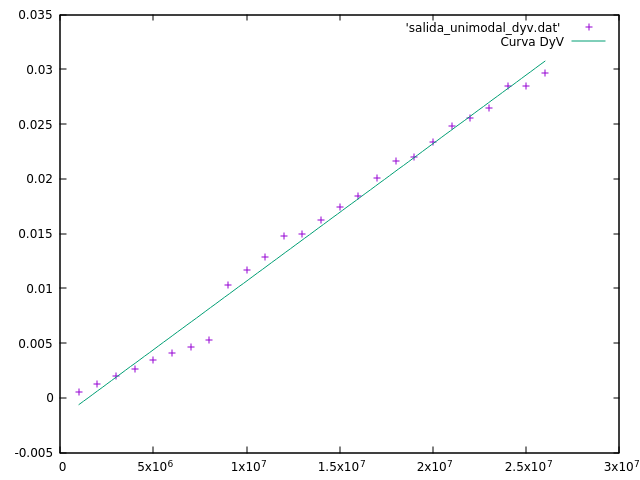
\includegraphics[angle=0,scale=0.5]{img/AjusteHibridoDyV.png} 
\caption{Ajustada a la función $f(x)=a_0*log(x)+a_1*x+a_2$} 
\end{figure}

\end{frame}

\begin{frame}
\[
f(x)=a_0*log(x)+a_1*x+a_2
\]
\[
a_0=1.75072e-09
\]
\[
a_1=1.24488e-10
\]
\[
a_2=0.000151147 
\]
\end{frame}

\begin{frame}{Correlación}
\begin{itemize}
\item Unimodal secuencial:

	Coeficiente de correlación en el caso lineal: \\
	0,999967757\\
	Coeficiente de correlación en el caso logarítmico: 
	0,999967634
	
\vspace{3mm} %5mm vertical space

\item Unimodal Divide y Vencerás:

	Coeficiente de correlación en el caso lineal: \\
	0,993561274\\
	Coeficiente de correlación en el caso logarítmico: 
	0,99566217
	
\vspace{5mm} %5mm vertical space

En el caso secuencial el ajuste lineal es mejor, mientras que en Divide y Vencerás el mejor ajuste es el logarítmico. 
\end{itemize}
\end{frame}

\begin{frame}{Conclusión}
Como podemos observar, el mismo problema se puede resolver de forma más rápida y eficiente si empleamos un algoritmo de tipo Divide y Vencerás que uno secuencial.
\vspace{5mm} %5mm vertical space
En este caso con Divide y Vencerás podemos conseguir que la eficiencia del algoritmo pase de ser $O(n)$ a $O(log n)$, por lo que somos capaces de procesar muchos más datos en un tiempo menor. 
\vspace{5mm} %5mm vertical space
De esta forma se puede concluir que siempre que vayamos a usar datos lo bastante grandes es mejor realizar el algoritmo mediante Divide y Vencerás que mediante uno secuencial. 
\end{frame}

\end{document}
\grid
